%\documentclass[onecolumn]{IEEEtranTIE}
\documentclass[journal]{IEEEtranTIE}

\usepackage{graphicx}
\usepackage{cite}
\usepackage{picinpar}
\usepackage{amsmath}
\usepackage{url}
\usepackage{flushend}
\usepackage[latin1]{inputenc}
\usepackage{colortbl}
\usepackage{soul}
\usepackage{multirow}
\usepackage{pifont}
\usepackage{color}
\usepackage{alltt}
\usepackage[hidelinks]{hyperref}
\usepackage{enumerate}
\usepackage{siunitx}
\usepackage{breakurl}
\usepackage{epstopdf}
\usepackage{pbox}

\usepackage{booktabs}
\usepackage{amsmath}
\usepackage{amssymb}
\usepackage{algorithmicx}
\usepackage{algpseudocode}
\renewcommand{\algorithmicrequire}{\textbf{Input:}}
\renewcommand{\algorithmicensure}{\textbf{Output:}}


\begin{document}
\title{	Preparation of Papers for IEEE Trans on Industrial Electronics \\ (Nov. 2020)}

\author{
	\vskip 1em
	
	First A. Author1, \emph{Student Membership},
	Second B. Author2, \emph{Membership},
	\\ and Third C. Author3, \emph{Membership}

	\thanks{
	
		Manuscript received Month xx, 2xxx; revised Month xx, xxxx; accepted Month x, xxxx.
		This work was supported in part by the xxx Department of xxx under Grant  (sponsor and financial support acknowledgment goes here).
		
		(Authors' names and affiliation) First A. Author1 and Second B. Author2 are with the xxx Department, University of xxx, City, Zip code, Country, on leave from the National Institute for xxx, City, Zip code, Country (e-mail: author@domain.com). 
		
		Third C. Author3 is with the National Institute of xxx, City, Zip code, Country (corresponding author to provide phone: xxx-xxx-xxxx; fax: xxx-xxx-xxxx; e-mail: author@ domain.gov).
	}
}

\maketitle
	
\begin{abstract}
Paper titles should be written in uppercase and lowercase letters, not all uppercase. Avoid writing long formulas with subscripts in the title; short formulas that identify the elements are fine (e.g., ``Nd-Fe-B''). Do not write ``(Invited)'' in the title. Write full names of authors in the author field. Define all symbols used in the abstract. Do not cite references in the abstract. Do not delete the blank line immediately above the abstract; it sets the footnote at the bottom of this column.
\end{abstract}

\begin{IEEEkeywords}
??? Enter key words or phrases in alphabetical order, separated by commas.
\end{IEEEkeywords}

\markboth{IEEE TRANSACTIONS ON INDUSTRIAL ELECTRONICS}%
{}

\definecolor{limegreen}{rgb}{0.2, 0.8, 0.2}
\definecolor{forestgreen}{rgb}{0.13, 0.55, 0.13}
\definecolor{greenhtml}{rgb}{0.0, 0.5, 0.0}

\section{Important information}

\IEEEPARstart{T}{his} ???

Regular Papers and Special Section papers - Four to eight pages, including authors' bios and photos.

\begin{enumerate}[1)]
	\item New manuscripts cannot exceed \textbf{8 pages} (3 for letters). Only a very limited overlength (1/2 page at most) is tolerated. Note that usually in the review process the reviewers tend to ask for more explanations, also note that the maximum allowed length is 8 pages on initial/first submission, including authors' bios and photos.
	\item In order to follow the \textbf{single-blind} review process, we ask that all the authors be identifiable within the manuscript (DO include authors' names, their biographies, affiliation, etc.). Each published article was reviewed by a minimum of two independent reviewers using a single-blind peer review process.
	\item The only file which has to be submitted (uploaded) is the \textbf{manuscript in PDF format}.
	\item IEEE T IE is an application oriented engineering journal. It is therefore expected that all submissions will \textbf{contain experimental verification} of the novel theoretical concepts, given in the paper. Papers not containing experimental results should therefore not be submitted since they will be subject to an ``Immediate reject'' decision. An experimental rig, which must be used by the authors for verification, must contain hardware components other than a PC/laptop.	
\end{enumerate}

Figures that are composed of only black lines and shapes. These figures should have no shades or half-tones of gray. Only black and white.

The final printed size of author photographs is exactly
1 inch wide by 1.25 inches tall (25.4 millimeters x 31.75 millimeters / 6 picas x 7.5 picas).

When referencing your figures and tables within your paper, use the abbreviation ``Fig.'' even at the beginning of a sentence. Do not abbreviate ``Table.'' Tables should be numbered with Roman Numerals.

The IEEE Graphics Checker Tool enables authors to pre-screen their graphics for compliance with IEEE Transactions and Journals standards before submission. The online tool, located at \url{http://graphicsqc.ieee.org/}, allows authors to upload their graphics in order to check that ... 

A conclusion section is not required. Although a conclusion may review the main points of the paper, do not replicate the abstract as the conclusion. A conclusion might elaborate on the importance of the work or suggest applications and extensions.

Reference numbers are set flush left and form a column of their own, hanging out beyond the body of the reference. The reference numbers are on the line, enclosed in square brackets. In all references, the given name of the author or editor is abbreviated to the initial only and precedes the last name. Use them all; use et al. exceptionally if more than 6 author names were listed. Use commas around Jr., Sr., and III in names. 

Other than books \cite{inbook1, book1, book2, book3}, capitalize only the first word in a paper title, except for proper nouns and element symbols. 

Because replication is required for scientific progress, papers submitted for publication must provide sufficient information to allow readers to perform similar experiments or calculations and use the reported results. Although not everything need be disclosed, a paper must contain new, useable, and fully described information.

\newpage





\section{Introduction}

Text of the introduction.
\begin{itemize}
\item minimum effort control - minimizing the control effort, where the
effort is defined as maximum amplitude of the control \cite{neustadt1962minimum,porter1966note,Tomlin1975}
\item minimum effort control in robotics (kinematically redundant manipulators)
\cite{ajoudani2013human,lee2001structured,Shim1998,Lee&Ha2001}, 
\item traditional control methods of power converters, carrier-based PWM
techniques (sinusoidal, TIPWM) and space vector-based techniques (SVPWM).
\end{itemize}

\section{Motivation and principles}

\subsection{Redundant Voltage Source Network }

The problem of redundant voltage source network, degrees of freedom.
Analogy to voltage source converters. Clarke's transform, A matrix,
vector x as a vector of final voltages with minimum amplitudes.

\begin{equation}
\begin{aligned}x=\left[\cdots\right]{}^{T},\\
A=\left[\cdots\right],
\end{aligned}
\label{eq:eq2-1}
\end{equation}
Motivation -> minimize voltage needed.

\subsection{Optimization problem definition}

Linear system, minimum infinity norm, solution vector x. Primal problem
definition...

\begin{equation}
\min_{\mathbf{Ax}=\mathbf{y}}||\mathbf{x}||_{\text{\ensuremath{\infty}}},\label{eq:1}
\end{equation}


\subsection{Solution using linear programming???}

Note sure if this is to include in the paper......Solution using linear
programming - linprog() in Matlab environment, suitable for mathematical
modeling and rapid method development for any type of converter. Not
effective for real-time application...

\section{Proposed Solution}

\subsection{Solution way for m (m + 1) matrices}

..... 

If matrix A is of size m (m + 1) and if its rank is m (its rows are
independent), then we have 

fx j Ax = yg = fx0 + sa j s 2 Rg; where x0 is an arbitrary point which
satises Ax0 = y and a is a nonzero element of kernel of A (it satises
Aa = 0). Then (1) is equivalent to minimize x;s kxk1 subject to x
= x0 + sa; which amounts solving an optimization problem in one dimension
minimize s kx0 + sak1: (3) For the the optimal solution of (3), there
will be some indices i 6= j such that the components satisfy (x0 +
sa)i = (x0 + sa)j : This have two solutions (if properly dened)

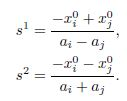
\includegraphics{Figures/temp3}

Then among all these s, we select the one with minimal kx0+sak1. We
summarize the procedure in Algorithm 1.1.

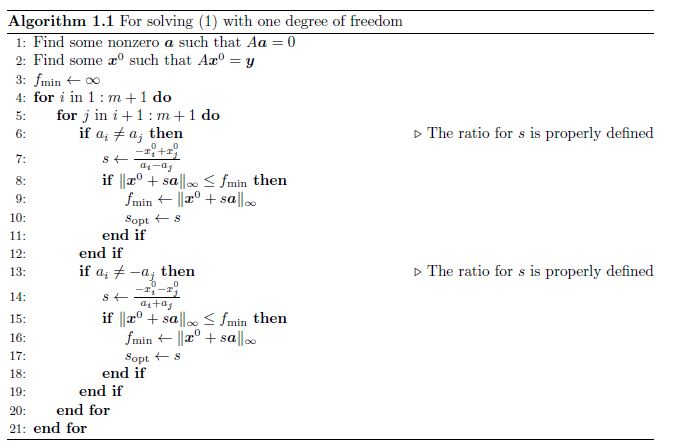
\includegraphics[width=0.9\columnwidth]{Figures/temp}

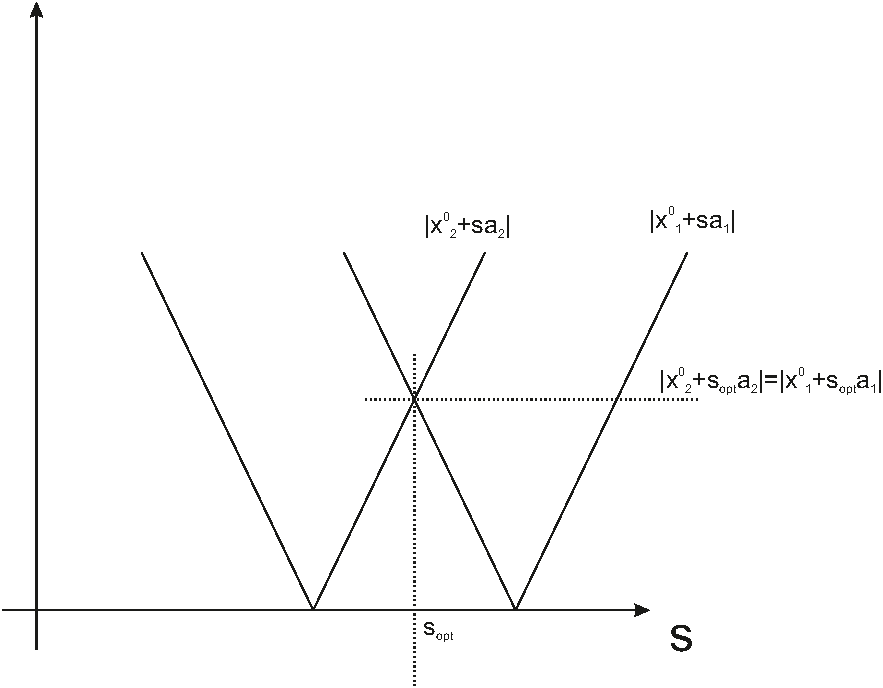
\includegraphics[width=0.9\columnwidth]{Figures/ilust_obr_x0+sa}

\subsection{Solution way for a general matrix A}

....

When A is of a dierent size, then the kernel is no longer a line but
a more dimensional spaces whose dimension equals to the degree of
freedom. Denote the generators of this space by a1; : : : ; aK. Then
we have again

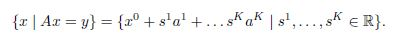
\includegraphics{Figures/temp2}

This means that (3) is replaced by

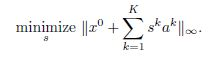
\includegraphics{Figures/temp1}

...

Solution by ADMM

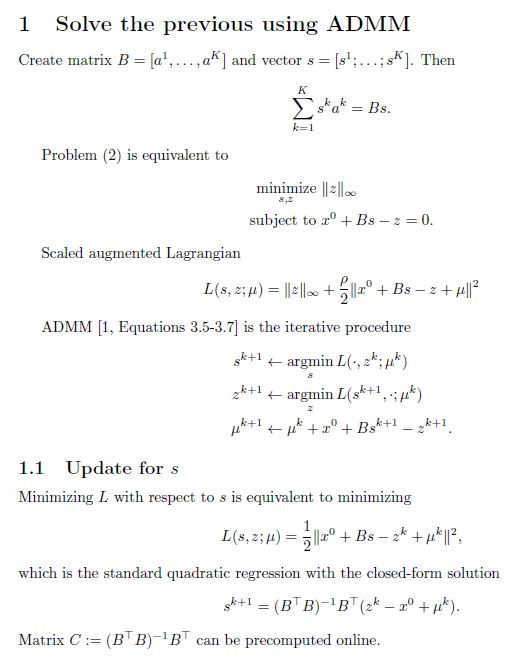
\includegraphics[width=0.9\columnwidth]{Figures/temp4}

...

...Problem solving requires high processing power, not very effective
in real-time environment....

\subsection{Solution of Dual Problem}

... Duality of $\ell_{1}$ and $\ell_{\infty}$ norm (D. G. Luenberger)
\cite{Luenberger1997optimization}. Dual problem defined by Cadzow:

The Cadzow algorithm \cite{Cadzow1973,Cadzow1974efficient} is based
on a solution search of the associated dual problem 
\begin{equation}
\max_{\left\Vert \mathbf{A}^{T}\mathbf{u}\right\Vert _{1}\leqq1}\mathbf{y}^{T}\mathbf{u}=\min_{\mathbf{Ax}=\mathbf{y}}||\mathbf{x}||_{\text{\ensuremath{\infty}}},\label{eq:6}
\end{equation}
using the alignment property between final vectors $\mathbf{A}^{T}\mathbf{u}^{0}$
and $\mathbf{x}^{0}$ to evaluate $\mathbf{x}^{0}$:

\begin{equation}
\left[\mathbf{A}^{T}\mathbf{u}^{0}\right]^{T}\mathbf{x}^{0}=\left\Vert \mathbf{A}^{T}\mathbf{u}^{0}\right\Vert _{1}\left\Vert \mathbf{x}^{0}\right\Vert _{\infty},
\end{equation}
i.e. 
\begin{equation}
\left\Vert \mathbf{x}^{0}\right\Vert _{\infty}=\mathbf{y}^{T}\mathbf{u}^{0}=\left[\mathbf{A}^{T}\mathbf{u}^{0}\right]^{T}\mathbf{x}^{0}.
\end{equation}
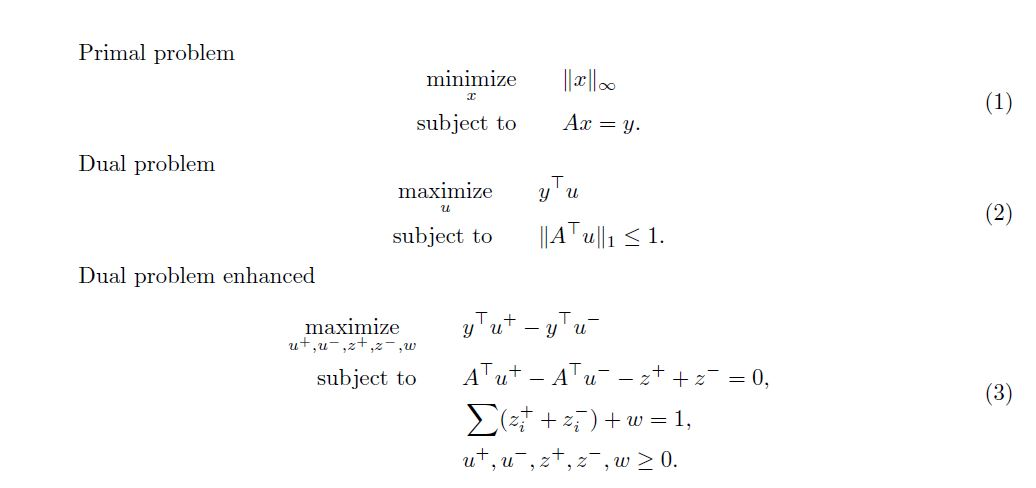
\includegraphics[width=0.9\columnwidth]{Figures/temp5}

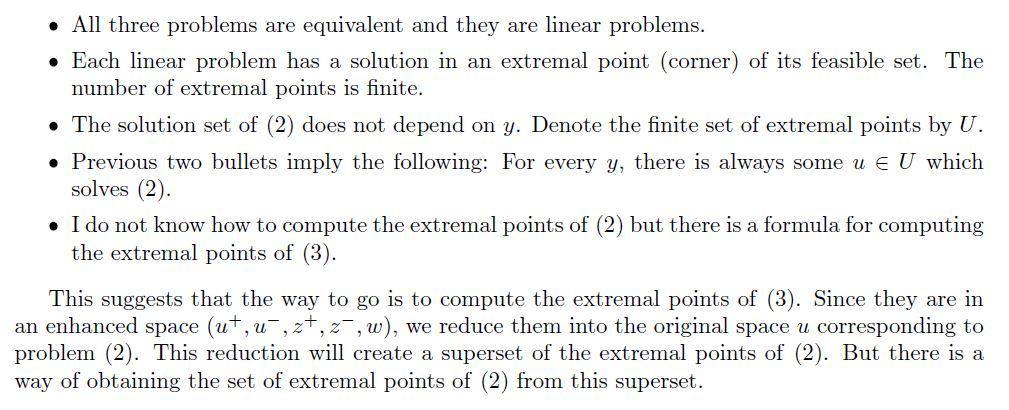
\includegraphics[width=0.9\columnwidth]{Figures/temp6}

\begin{figure}
\noindent \begin{centering}
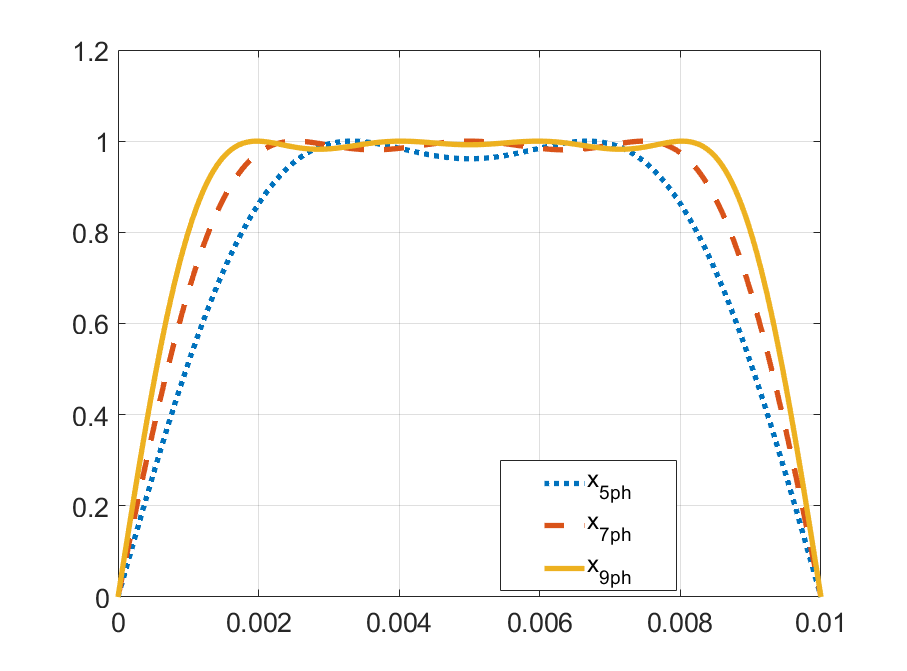
\includegraphics[width=6cm]{Figures/optimized_flux_waveform_5_7_9ph}
\par\end{centering}
\caption{\label{fig:optimal-ratio-harmonics} Figure example}
\end{figure}


\section{Application/Control of Power Converters)}

\subsection{Traditional three-phase converters}

Conventional three-phase converters, correlation to SVPWM and 

\subsection{Three-phase four-leg converters}

Text text text. Text text text. Text text text. Text text text. Text
text text. Text text text. Text text text. Text text text. Text text
text. Text text text. Text text text. Text text text. Text text text.
Text text text. Text text text. Text text text. Text text text. Text
text text. Text text text. Text text text. Text text text.

\subsection{Multilevel converters}

Text text text. Text text text. Text text text. Text text text. Text
text text. Text text text. Text text text. Text text text. Text text
text. Text text text. Text text text. Text text text. Text text text.
Text text text. Text text text. Text text text. Text text text. Text
text text. Text text text. Text text text. Text text text.

\subsection{Multiphase converters}

Text text text. Text text text. Text text text. Text text text. Text
text text. Text text text. Text text text. Text text text. Text text
text. Text text text. Text text text. Text text text. Text text text.
Text text text. Text text text. Text text text. Text text text. Text
text text. Text text text. Text text text. Text text text.

\section{Experimental results}

Some experimental results.\textcolor{red}{}
\begin{figure}
\begin{centering}
\textcolor{red}{}%
\begin{tabular}{>{\centering}p{4.2cm}>{\centering}p{4.2cm}}
\textcolor{red}{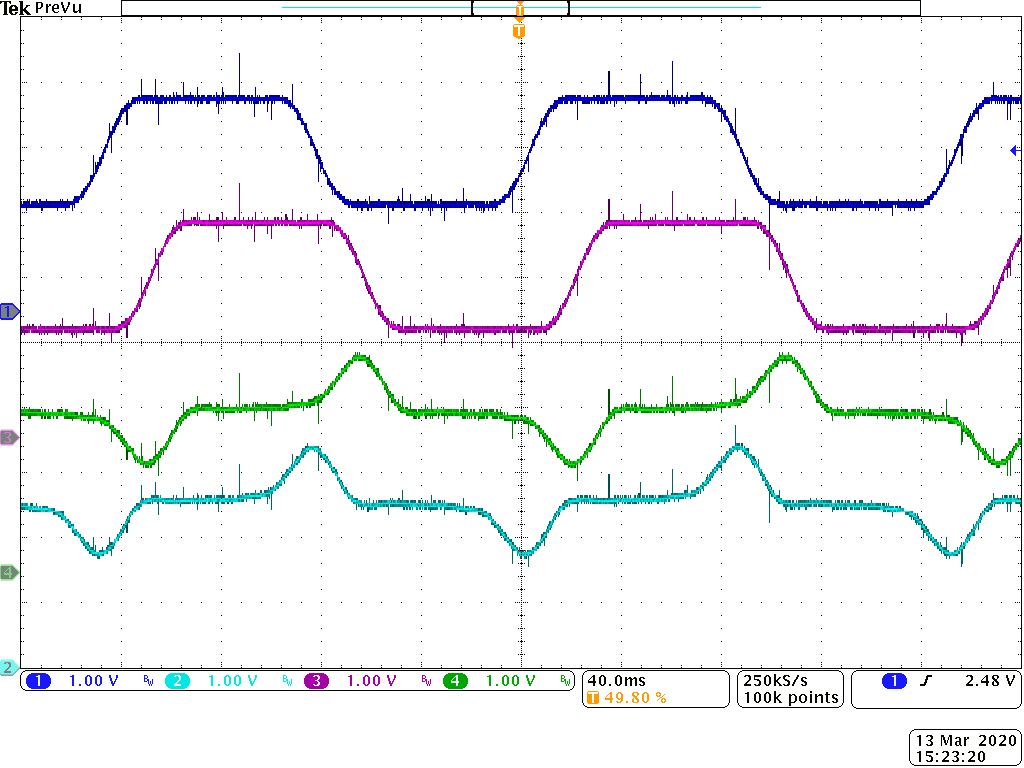
\includegraphics[width=0.48\columnwidth]{Figures/tek00002}} & \textcolor{red}{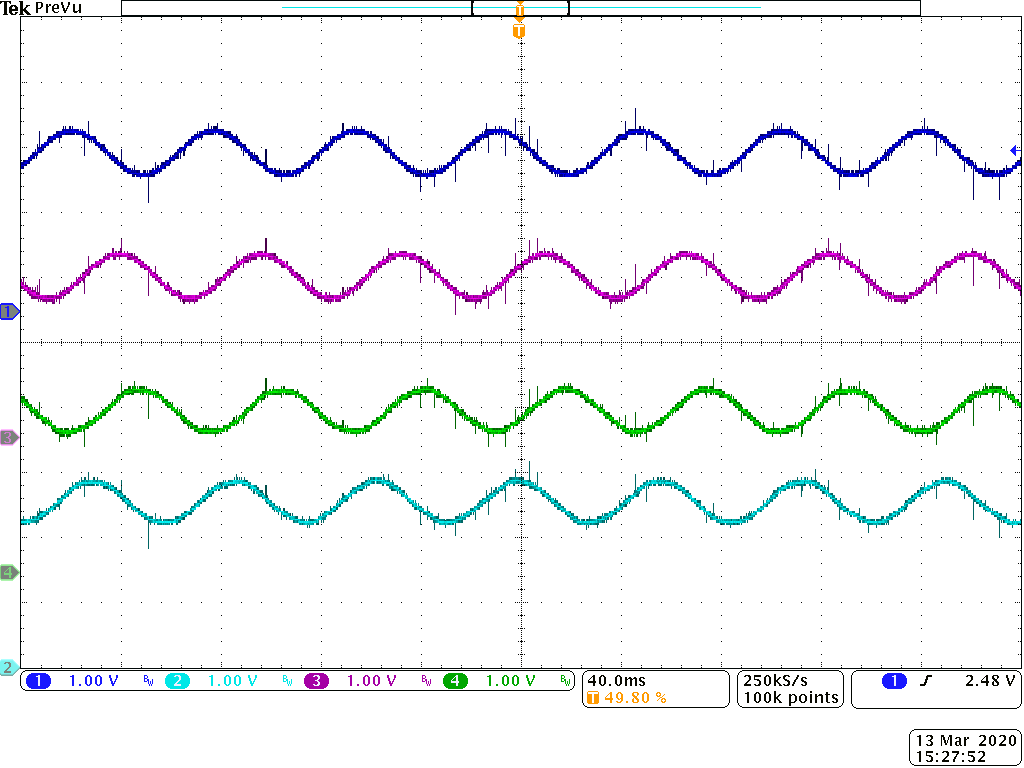
\includegraphics[width=0.48\columnwidth]{Figures/tek00002x}}\tabularnewline
 & \tabularnewline
{\footnotesize{}(a) Fundamental with 3\textsuperscript{rd} , 5\textsuperscript{th}
, and 7\textsuperscript{th} harmonic component.} & {\footnotesize{}(b) 3\textsuperscript{rd}harmonic component only.}\tabularnewline
\end{tabular}
\par\end{centering}
\caption{\label{fig:exp-results-1} Example of experimental results}
\end{figure}
\textcolor{red}{{} }

\section{Conclusion}

Conclusion Text text text. Text text text. Text text text. Text text
text. Text text text. Text text text. Text text text. Text text text.
Text text text. Text text text..






\appendix


\section*{???}


\section*{Acknowledgment}



\bibliographystyle{Bibliography/IEEEtranTIE}
\bibliography{Bibliography/ref}
%\bibliography{Bibliography/IEEEabrv,Bibliography/BIB_xx-TIE-xxxx}\ %IEEEabrv instead of IEEEfull

	
	
%\vspace{-1cm}
\begin{IEEEbiography}[{
\includegraphics[width=1in,height=1.25in,clip,keepaspectratio]{Figures/photo-men.eps}}]
{First A. Author1} and the other authors may include biographies at the end of regular papers. The first paragraph may contain a place and/or date of birth (list place, then date). Next, the author's educational background is listed. The degrees should be listed with type of degree in what field, which institution, city, state or country, and year degree was earned. The author's major field of study should be lower-cased.

The second paragraph uses the pronoun of the person (he or she) and not the author's last name. It lists military and work experience, including summer and fellowship jobs. Job titles are capitalized. The current job must have a location; previous positions may be listed without one. Information concerning previous publications may be included.

The third paragraph begins with the author's title and last name (e.g., Dr. Smith, Prof. Jones, Mr. Kajor, Ms. Hunter). List any memberships in professional societies other than the IEEE. Finally, list any awards and work for IEEE committees and publications. If a photograph is provided, the biography will be indented around it. The photograph is placed at the top left of the biography. Personal hobbies will be deleted from the biography.
\end{IEEEbiography}



\end{document}
